\begin{figure}
    \centering
    \setlength{\resLen}{0.8in}
    \addtolength{\tabcolsep}{-3pt}
    \begin{tabular}{cccc}
        \multicolumn{4}{c}{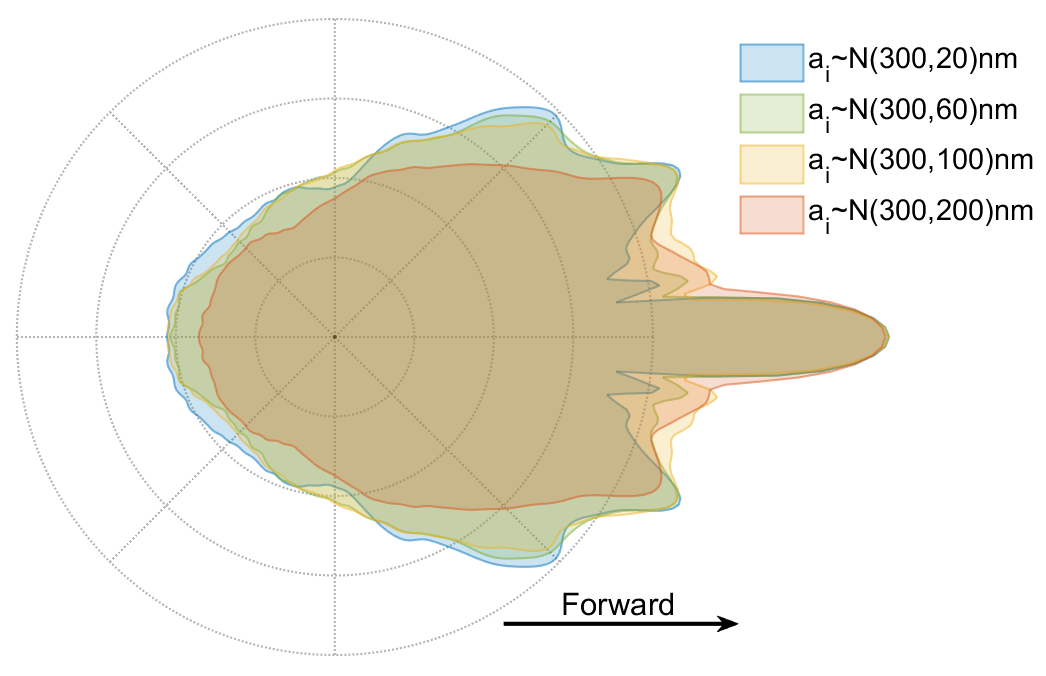
\includegraphics[height=1.8\resLen]{images/pfunc/radius_gaussian.png}}
        \\
        %
        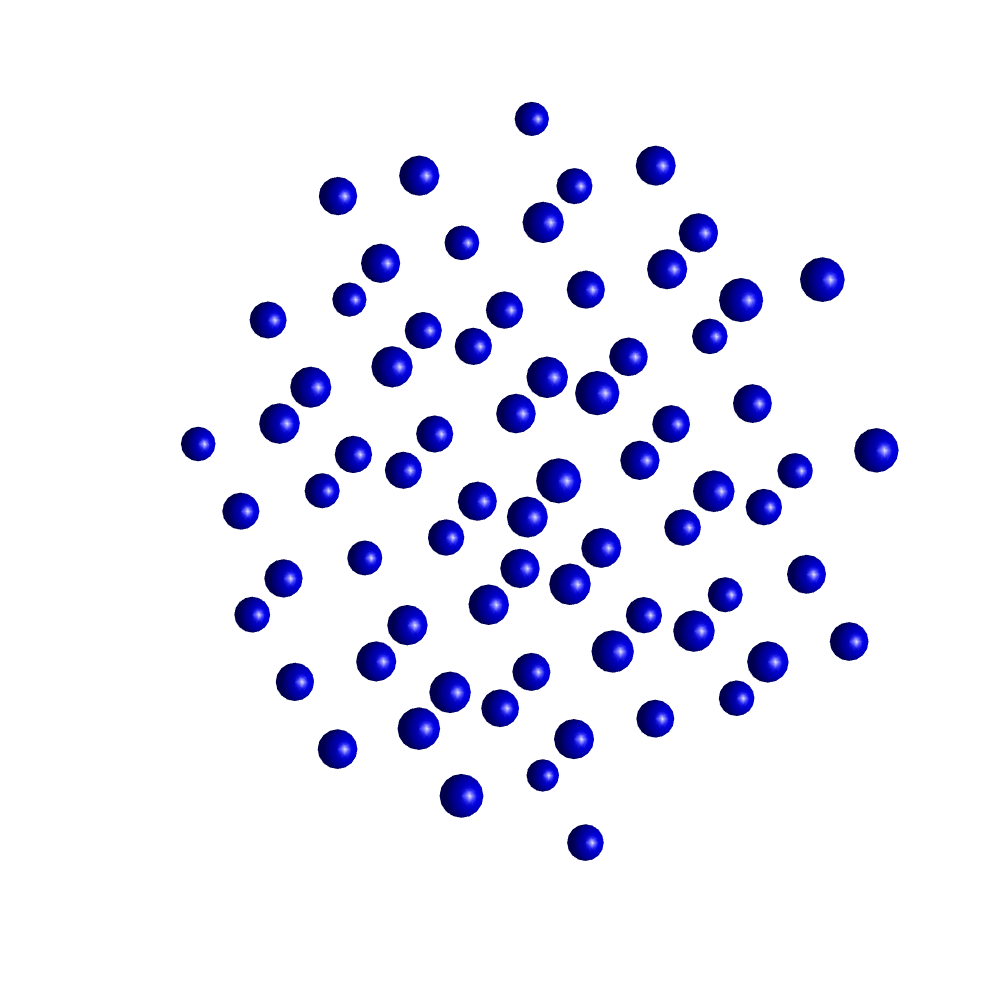
\includegraphics[width=\resLen]{images/particle/sigma_0.02.png} &
        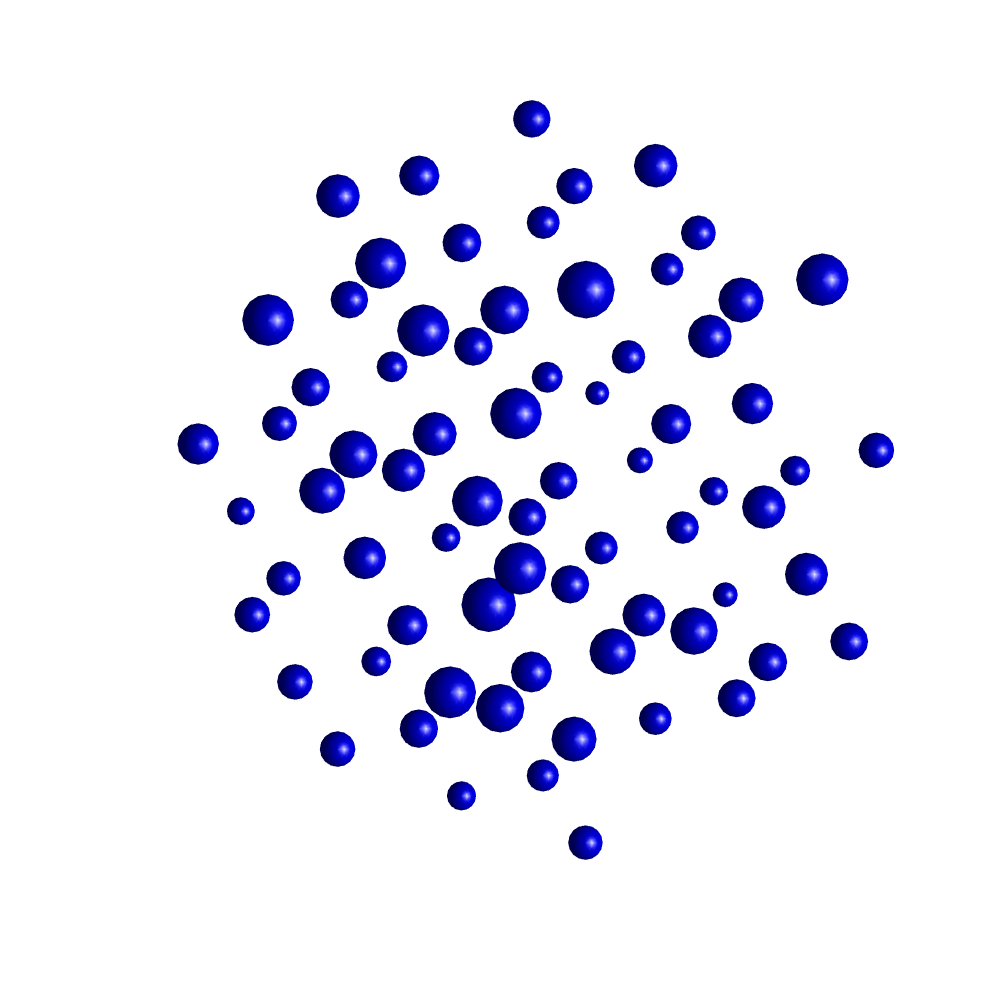
\includegraphics[width=\resLen]{images/particle/sigma_0.06.png} &
        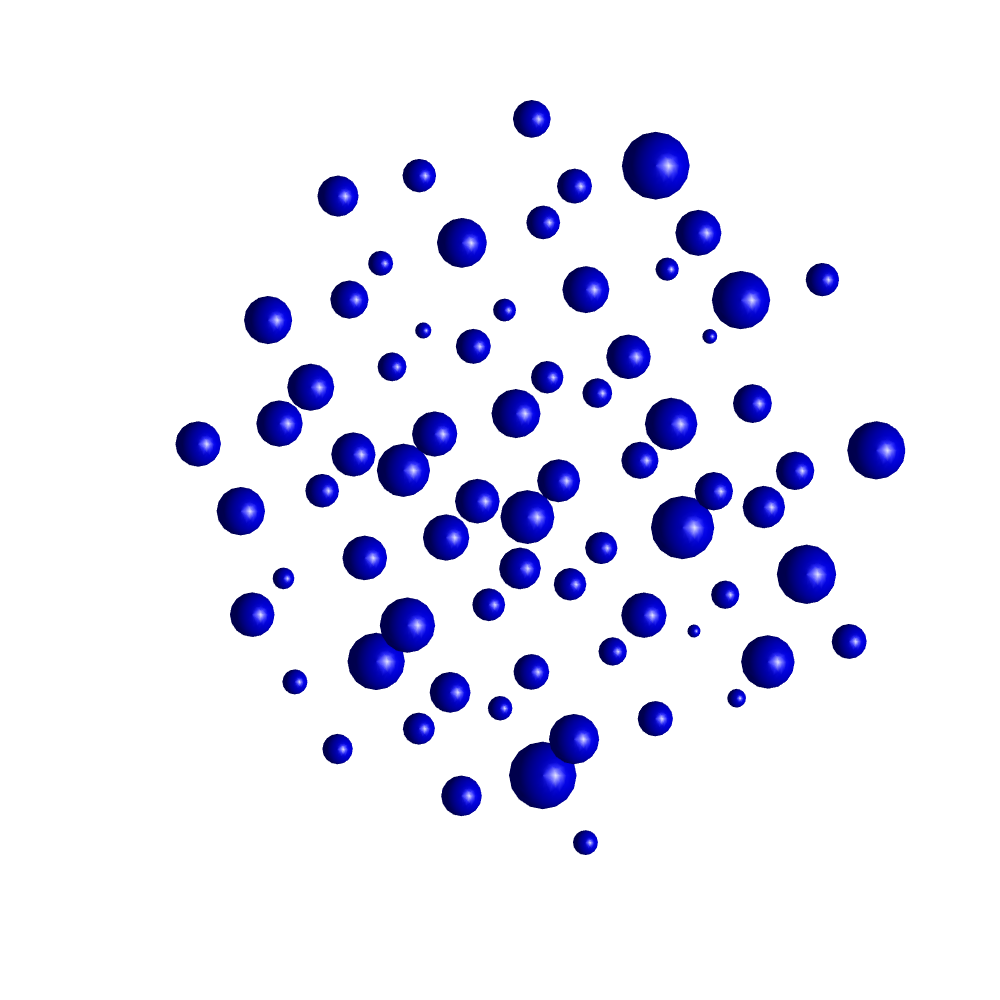
\includegraphics[width=\resLen]{images/particle/sigma_0.1.png} &
        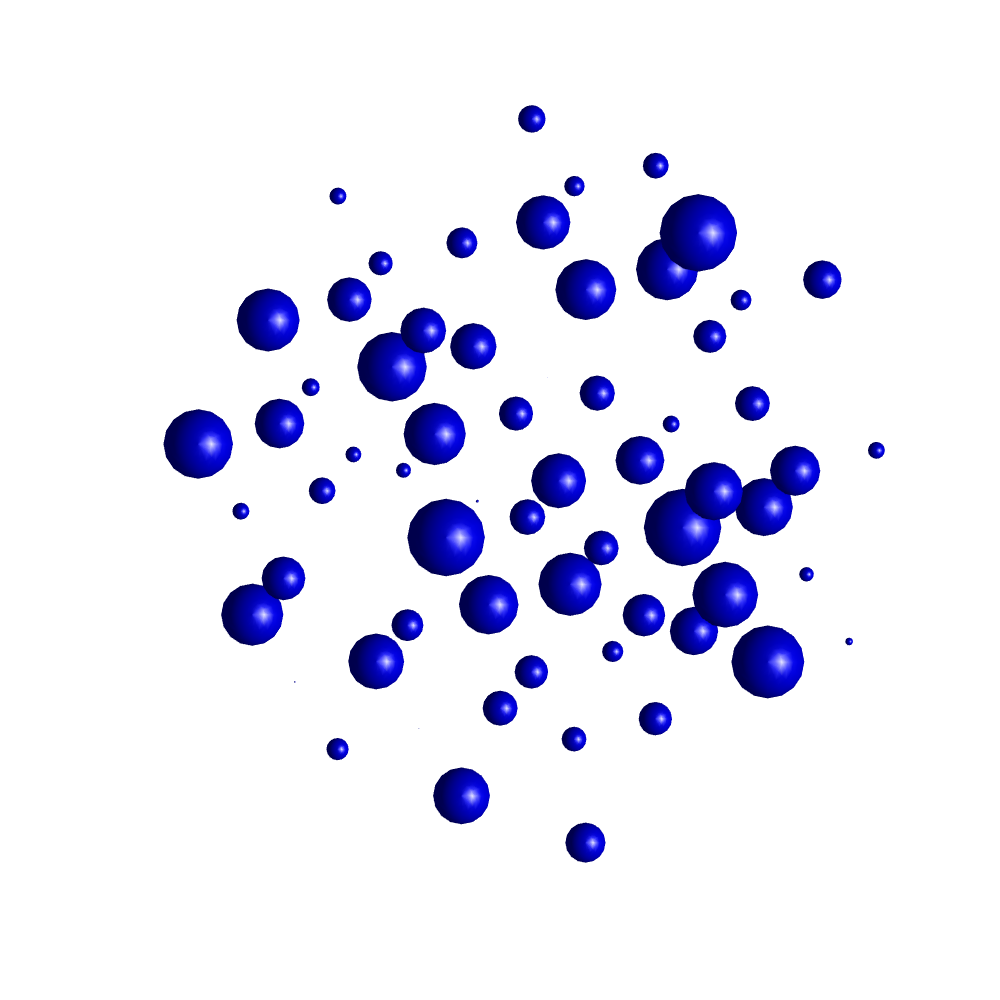
\includegraphics[width=\resLen]{images/particle/sigma_0.2.png}\\[-0.5em]
        %
        \begin{overpic}[width=\resLen]{images/lucy/sigma_0.02.jpg}
            % \put(0,0){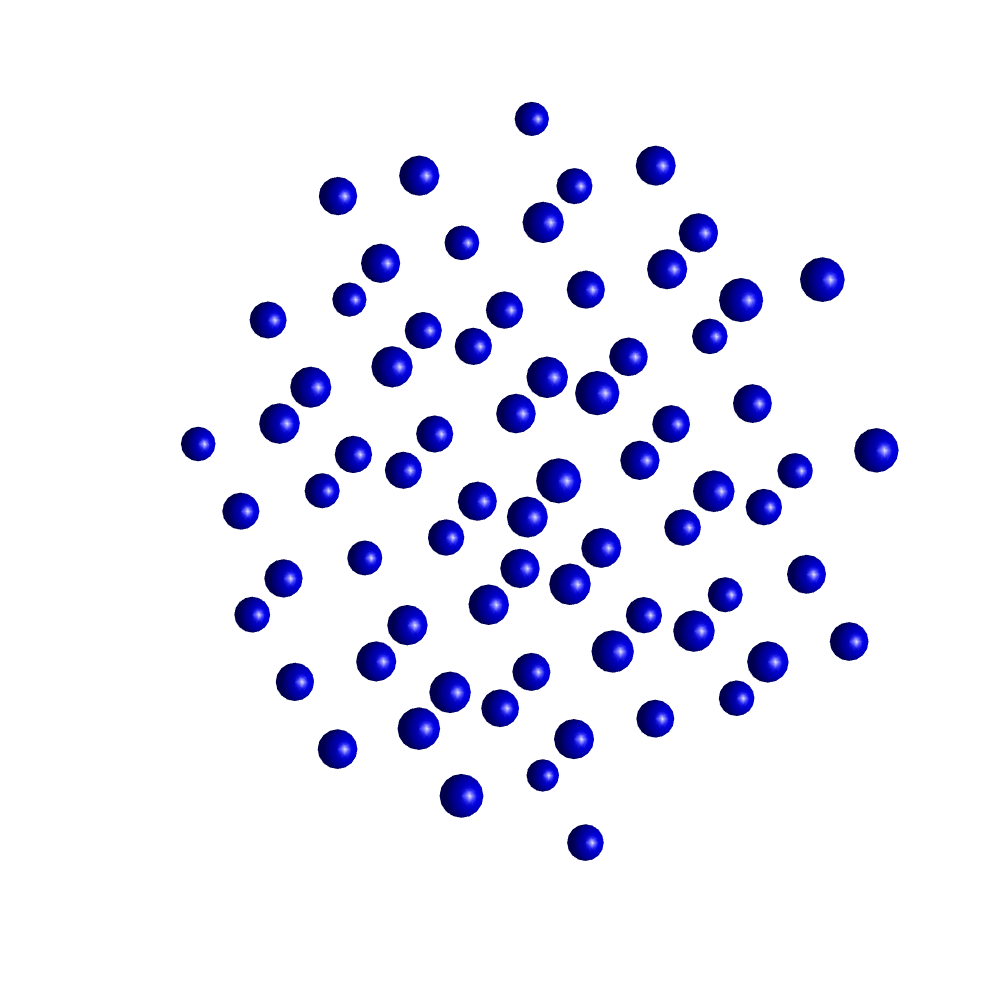
\includegraphics[width=.4\resLen]{images/particle/sigma_0.02.png}}
        \end{overpic}
        &
        \begin{overpic}[width=\resLen]{images/lucy/sigma_0.06.jpg}
            % \put(0,0){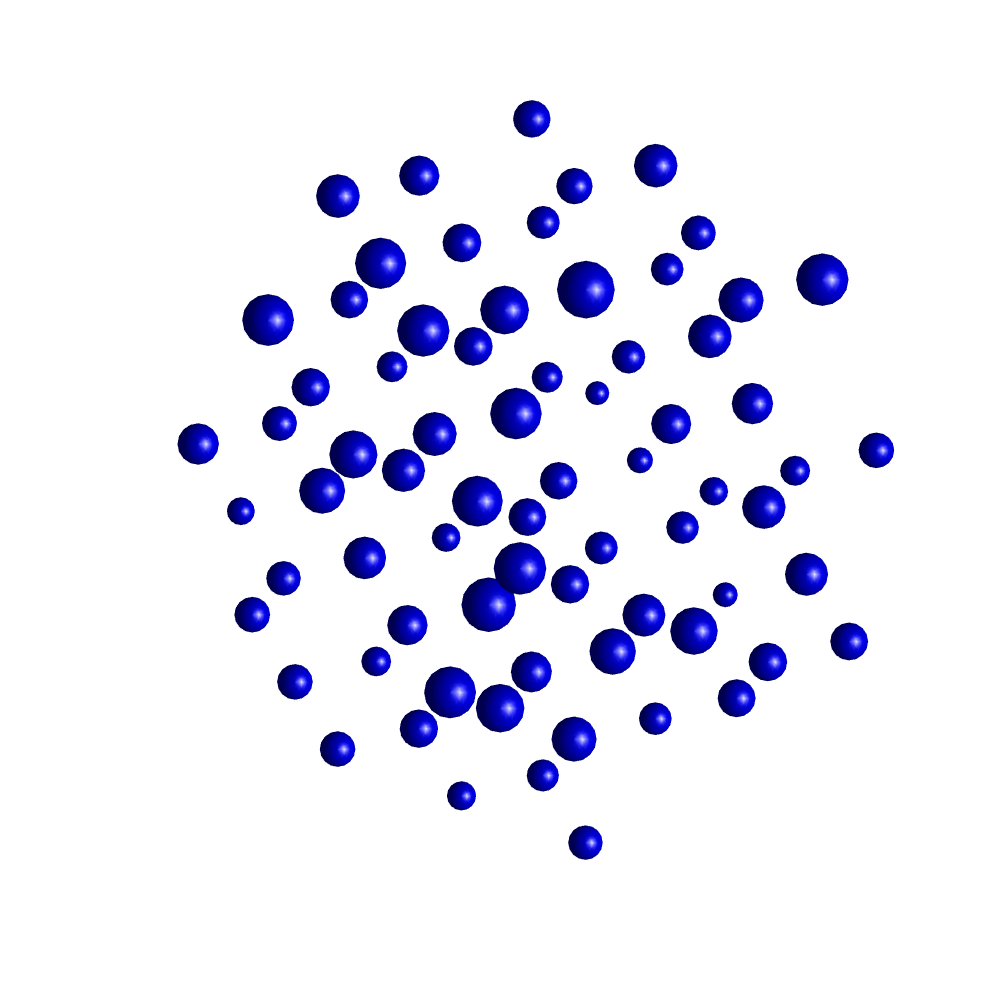
\includegraphics[width=.4\resLen]{images/particle/sigma_0.06.png}}
        \end{overpic}
        &
        \begin{overpic}[width=\resLen]{images/lucy/sigma_0.1.jpg}
            % \put(0,0){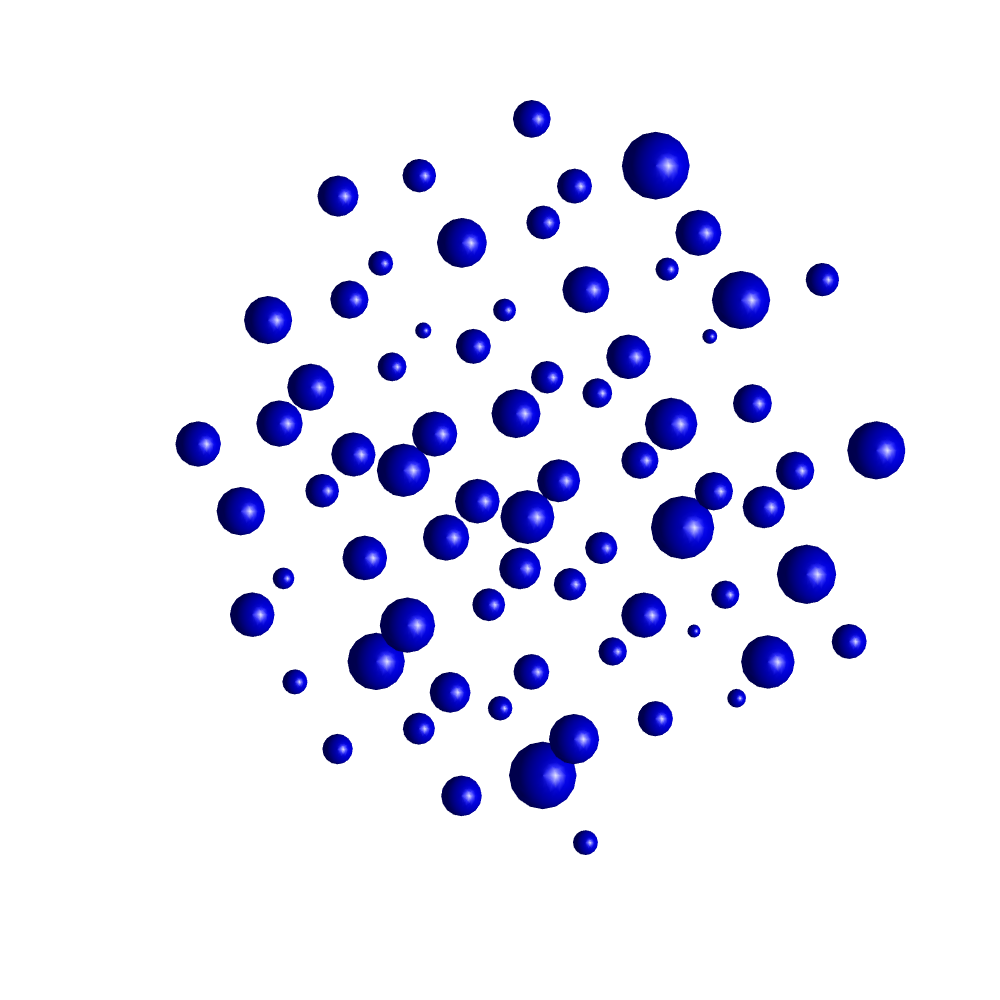
\includegraphics[width=.4\resLen]{images/particle/sigma_0.1.png}}
        \end{overpic}
        &
        \begin{overpic}[width=\resLen]{images/lucy/sigma_0.2.jpg}
            % \put(0,0){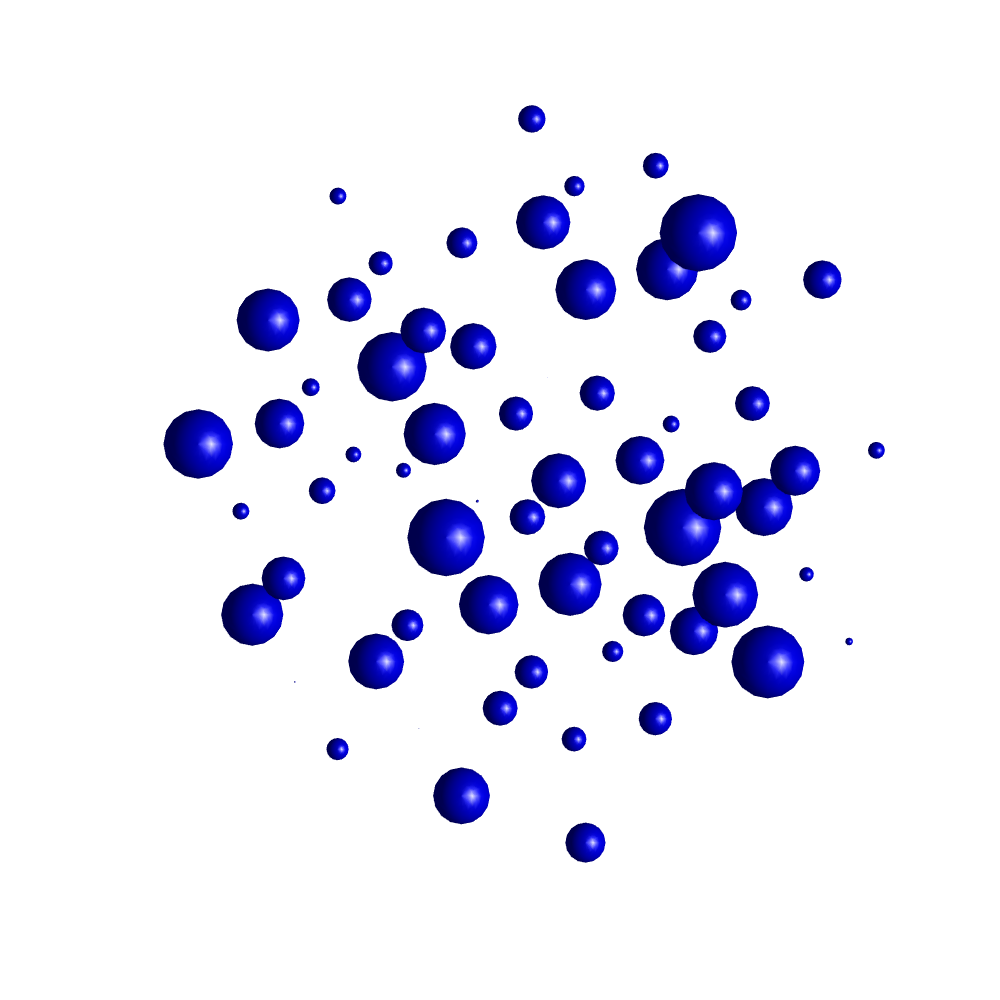
\includegraphics[width=.4\resLen]{images/particle/sigma_0.2.png}}
        \end{overpic}
        \\
        $\mathcal{N}(300,20)\,$nm & $\mathcal{N}(300,60)\,$nm & $\mathcal{N}(300,100)\,$nm & $\mathcal{N}(300,200)\,$nm
    \end{tabular}
    \caption{\label{fig:paritclesize}
        \rev{
            Our technique supports clusters comprised of particles with varying sizes.
            The top of this figure visualizes bulk phase functions of four media generated with $\Ncls = 100$ and uniformly distributed particles.
            Further, sizes of particles in each cluster are normally distributed with the same mean ($300$nm) but varying standard deviations ($20$nm, $60$nm, $100$nm, and $200$nm).
            The bottom of this figure shows renderings of the Lucy model made of the four media, respectively.
        }
        %\rev{Comparison of the resulting phase function and rendering for different particle radius distribution. They have the same mean radius but different variations.}
    }
\end{figure}

